%%%%%%%%%%%%%%%%%%%%%%%%%%%%%%%%%%%%%%%%%
% Dreuw & Deselaer's Poster
% LaTeX Template
% Version 1.0 (11/04/13)
%
% Created by:
% Philippe Dreuw and Thomas Deselaers
% http://www-i6.informatik.rwth-aachen.de/~dreuw/latexbeamerposter.php
%
% This template has been downloaded from:
% http://www.LaTeXTemplates.com
%
% License:
% CC BY-NC-SA 3.0 (http://creativecommons.org/licenses/by-nc-sa/3.0/)
%
%%%%%%%%%%%%%%%%%%%%%%%%%%%%%%%%%%%%%%%%%

%----------------------------------------------------------------------------------------
%	PACKAGES AND OTHER DOCUMENT CONFIGURATIONS
%----------------------------------------------------------------------------------------

\documentclass[final,hyperref={pdfpagelabels=false}]{beamer}

\usepackage[orientation=portrait,size=a0,scale=1.4]{beamerposter} % Use the beamerposter package for laying out the poster with a portrait orientation and an a0 paper size

\usetheme{I6pd2} % Use the I6pd2 theme supplied with this template

\usepackage[english]{babel} % English language/hyphenation

\usepackage{amsmath,amsthm,amssymb,latexsym} % For including math equations, theorems, symbols, etc

\usepackage{subfigure}
%\usepackage{caption}
%\setbeamertemplate{caption}{\raggedright\insertcaption\par}

%\usepackage{times}\usefonttheme{professionalfonts}  % Uncomment to use Times as the main font
%\usefonttheme[onlymath]{serif} % Uncomment to use a Serif font within math environments

\boldmath % Use bold for everything within the math environment

\usepackage{booktabs} % Top and bottom rules for tables

\graphicspath{{figures/}} % Location of the graphics files

\usecaptiontemplate{\small\structure{\insertcaptionname~\insertcaptionnumber: }\insertcaption} % A fix for figure numbering

%----------------------------------------------------------------------------------------
%	TITLE SECTION 
%----------------------------------------------------------------------------------------

\title{\huge Surgical Activity Recognition in the Operating Room using RGBD Cameras} % Poster title

\author{Emre Ozan Alkan$^{1}$ - Supervisors: Andru Putra Twinanda$^{2}$, Nicolas Padoy$^{2}$} % Author(s)
%\author{Emre Ozan Alkan}

%\institute{}


\institute{Masters in Computer Vision, University of Burgundy}

% \institute{$^{1}$Masters in Computer Vision, University of Burgundy\\$^{2}$ICube, University of Strasbourg, CNRS,IHU Strasbourg, France} % Institution(s)

%----------------------------------------------------------------------------------------
%	FOOTER TEXT
%----------------------------------------------------------------------------------------

% \institute{$^{1}$Masters in Computer Vision, University of Burgundy\\$^{2}$ICube, University of Strasbourg, CNRS,IHU Strasbourg, France} % Institution(s)

\newcommand{\leftfoot}{$^{1}$Masters in Computer Vision, University of Burgundy $\bullet$ $^{2}$ICube, University of Strasbourg, CNRS,IHU Strasbourg, France}

%\newcommand{\leftfoot}{emreozanalkan.github.io} % Left footer text

%\newcommand{\rightfoot}{emreozanalkan@gmail.com} % Right footer text
\newcommand{\rightfoot}{ } % Right footer text

%----------------------------------------------------------------------------------------

\begin{document}

\addtobeamertemplate{block end}{}{\vspace*{2ex}} % White space under blocks

\begin{frame}[t] % The whole poster is enclosed in one beamer frame

\begin{columns}[t] % The whole poster consists of two major columns, each of which can be subdivided further with another \begin{columns} block - the [t] argument aligns each column's content to the top

\begin{column}{.02\textwidth}\end{column} % Empty spacer column

\begin{column}{.465\textwidth} % The first column

%----------------------------------------------------------------------------------------
%	OBJECTIVES
%----------------------------------------------------------------------------------------

% The objective of this study is to devise an efficient and accurate method for segmenting the hippocampus.
% The volume obtained from segmentation can be as a bio-marker to detect and track the progression
% of Alzheimer’s disease. However being a very small structure (3 to 5 mL) this process is challenging.

\begin{block}{Objectives}
% It is not a trivial problem because of various challenges. Firstly, camera positioning in operating rooms for better field of view while accommodating the articulation of the surgical equipments is very challenging. In addition, operating rooms are very dense and dynamic with a cluttered background and reflective objects, high occlusions, illumination changes , upfront camera view and very tiny or slow movements.
% Activity recognition is one of the key factors to enable the context-aware systems in the operating rooms.
Activity recognition is one of the key factors to enable the context-aware systems in the operating rooms (ORs). In this work, the problem of activity recognition from surgical video clips is addressed. It is not trivial problem due to camera positioning in an OR, cluttered background, reflective objects, occlusions and illumination changes. Multi-view RGBD cameras are used for acquisition.
% \begin{enumerate}
% 	\item Providing context-aware systems to ORs
%     \item Addressing the problem of activity recognition in an OR
%     \item It is not trivial problem due to camera positioning in an OR, cluttered background, reflective object, high occlusion, illumination changes and upfront camera view.
% \item Donec fringilla, velit id lobortis commodo, eros dui consectetur mi, ut interdum lorem dui sed mauris.
% \item Nulla ac nulla rhoncus est bibendum ullamcorper:
% \item Quisque vestibulum, nisl sit amet gravida ultricies dis parturient montes, nascetur ridiculus musobortis commodo, eros dui consectetur mi.
%\end{enumerate}

\end{block}

%----------------------------------------------------------------------------------------
%	INTRODUCTION
%----------------------------------------------------------------------------------------
            
\begin{block}{Methodology}

\begin{itemize}
\item Interest point detection from intensity and depth data: STIP (Spatio-temporal Interest Points) and DSTIP (Depth STIP)
\item Feature extraction: 250-dimensional HOF (Histograms of Optical Flow) and 800-dimensional DCSF (Depth Cuboid Similarity Feature)
\item Data-driven feature encoding \cite{twinanda2015data} by learning two dictionaries
	\begin{itemize}
    	\item Visual dictionary for encoding the visual features
        \item Spatio-temporal dictionary to place a non-rigid spatio-temporal grid to extract patches 
	\end{itemize}
\item Two-level classification using SVM and RF classifiers
    
%     Then, learnt spatio-temporal dictionary $\mathbf{D_{st}}$ is used to place a non-rigid spatio-temporal grid to divide the spatio-temporal space into patches $\{P^{1},...,P^{K_{st}}\}$. These local patches from the non-rigid layout are high dimensional 4D patches. 

% \item Donec fringilla, velit id lobortis commodo, eros dui consectetur mi, ut interdum lorem dui sed mauris. Duis id sem nunc, a pharetra odio. Phasellus posuere \alert{semper massa}, id bibendum ligula tristique at. Integer sit amet vulputate turpis. Sed erat lacus, faucibus at viverra et, mattis nec sem. Cras faucibus \alert{scelerisque} cursus. Opet volutpat ligula. Duis semper lorem eget dui dignissim porttitor. Nulla facilisi. In ullamcorper lorem quis dolor iaculis nec egestas enim ultricies. Cras ut mauris elit, ut lacinia dui. Proin in ante et libero hendrerit iaculis. Nulla eu erat a urna laoreet auctor id a turpis. Nam mollis tristique neque eu luctus. Suspendisse rutrum congue nisi sed convallis. Aenean id neque dolor.
\end{itemize}

\end{block}

%----------------------------------------------------------------------------------------
%	MATERIALS
%----------------------------------------------------------------------------------------

\begin{block}{Voting Scheme}

% We extended the pipeline aforementioned by proposing a voting scheme. The proposed voting scheme uses histograms $H^{j}$ obtained from patches $P^{j}$ of a data-driven non-rigid layout presented in Section~\ref{section:DataDrivenFeatureEncoding}. We classify every local patch $P^{j}$ using $H^{j}$ independently and collect their vote for calculating majority vote for global activity. Hence every patch $P^{j}$ holds information about activity with semantic information that is contributing globally. 

% In the first level, we learn a classification model to obtain the probability votes from the 4D patches. However, in the second level classification, we learn the weights for the probability votes under the assumption that each patch has different contribution.

\begin{columns} % Subdivide the first main column
\begin{column}{.54\textwidth} % The first subdivided column within the first main column
\begin{itemize}
\item The proposed voting scheme uses histograms obtained from patches of a data-driven non-rigid layout
\item Two-level classification in voting scheme
\begin{itemize}
\item 1st level: learning probability votes from the 4D patches
\item 2nd level: learning the weights for the probability votes
\end{itemize}
% \item Proin ut vestibulum augue.
% \begin{itemize}
% \item hopkop
% \end{itemize}
\end{itemize}
\end{column}

\begin{column}{.43\textwidth} % The second subdivided column within the first main column
\centering
\begin{figure}
\includegraphics[width=0.5\linewidth]{featureEncoding2.png}%{\\Figure caption}
%\caption{Figure caption}
\end{figure}

\begin{center}
{\small Data-driven non-rigid feature encoding}
\end{center}

\end{column}
\end{columns} % End of the subdivision

% \begin{itemize}
% \item Curabitur sapien ligula, faucibus in feugiat quis, vestibulum a turpis.
% \begin{itemize}
% \item Phasellus quis nunc neque. Suspendisse mauris diam, suscipit non gravida in, placerat id enim. Ut nec ipsum in lectus ultrices sagittis.
% \item Ut nec ipsum in lectus ultrices sagittis.
% \item Phasellus quis nunc neque.
% \end{itemize}
% \end{itemize}

\end{block}

%----------------------------------------------------------------------------------------
%	METHODS
%----------------------------------------------------------------------------------------

\begin{block}{Voting Scheme: One-Model Classification Approach}
\begin{itemize}
\item All patches are trained with one classifier in the first level
\end{itemize}

\begin{figure}
\includegraphics[width=1.0\linewidth]{figures/oneModelApproach3}%{\\Illustration of one-model approach to classify a video clip}
%\caption*{Illustration of one-model approach to classify a video clip}
\end{figure}

\begin{center}
{\small Illustration of one-model approach to classify a video clip}
\end{center}

% \begin{itemize}
% \item Maecenas Vel Nisl Elit
% \begin{itemize}
% \item Suspendisse potenti. Fusce a est eget turpis rhoncus varius sed sed dui. Cras justo nibh, bibendum a cursus eget, consequat et dui. Maecenas vel nisl elit, sed dignissim dolor. 
% \item In hac habitasse platea dictumst.
% \end{itemize}

% \item Viewpoint Matching Constraints
% \begin{itemize}
% \item Cum sociis natoque penatibus et magnis dis parturient montes, nascetur ridiculus mus. 
% \item Proin in nisi diam.
% \item Nam ultricies pellentesque nunc, ultrices volutpat nisl ultrices a.
% \end{itemize}

% \item Volutpat 
% \begin{itemize}
% \item Duis semper lorem eget dui dignissim porttitor.
% \item Nulla facilisi. In ullamcorper lorem quis dolor.
% \end{itemize}
% \end{itemize}

\end{block}

%----------------------------------------------------------------------------------------
%	MATHEMATICAL SECTION
%----------------------------------------------------------------------------------------

\begin{block}{Voting Scheme: Multi-Model Classification Approach}

\begin{itemize}
\item Each patch type has its own classifier in the first level
\end{itemize}

\begin{figure}
\includegraphics[width=1.0\linewidth]{figures/multiModelApproach3}%{\\Illustration of multi-model approach to classify a video clip}
%\caption*{Illustration of multi-model approach to classify a video clip}
\end{figure}

\begin{center}
{\small Illustration of multi-model approach to classify a video clip}
\end{center}

% \begin{itemize}
% \item Maecenas Ultricies Feugiat Velit Non Mattis.
% \item Fusce tempus arcu id ligula varius dictum.
% \item hophop
% \end{itemize}

% \begin{itemize}
% \item Maecenas Ultricies Feugiat Velit Non Mattis.
% \begin{itemize}
% \item Duis ante erat, bibendum nec tempus nec, interdum quis est. Nulla at mollis tortor. Phasellus quis leo dolor, aliquam laoreet orci $X$ Donec dapibus sagittis neque eu nec, interdum quis est. $Y_n, n=1,\cdots,N$ ndum nec tempus nec, interd
% \begin{align*}
% X \rightarrow r(X) & = \arg \max_{c} \Big\{ \max_n \big\{ \sum_{x_i \in X} \delta(x_i,Y_{n,c})\big\} \Big\} 
% \end{align*}
% \item Cras faucibus scelerisque cursus. Proin ut vestibulum augue. $\delta(x_i,Y_{n,c})$
% \end{itemize}
% \item Fusce tempus arcu id ligula varius dictum. Donec ut nisl dui, ac consectetur elit. In nec enim porta augue venenatis sollicitudin. Phasellus quis nunc neque. Suspendisse mauris diam, suscipit non gravida in, placerat id enim. Ut nec ipsum in lectus ultrices sagittis.
% \end{itemize}

\end{block}

%----------------------------------------------------------------------------------------

\end{column} % End of the first column

\begin{column}{.03\textwidth}\end{column} % Empty spacer column
 
\begin{column}{.465\textwidth} % The second column

%----------------------------------------------------------------------------------------
%	RESULTS
%----------------------------------------------------------------------------------------

\begin{block}{Dataset \cite{twinanda2015data}}

\begin{figure}
\centering
\subfigure[Camera view 1 - intensity data]{\label{sfig:view1Intensity}\includegraphics[scale=0.45]{figures/View1Color}}
\subfigure[Camera view 1 - depth data] {\label{sfig:view1Depth}\includegraphics[scale=0.45]{figures/View1Depth}}
\subfigure[Camera view 2 - intensity data]{\label{sfig:view1Intesity}\includegraphics[scale=0.45]{figures/View2Color}}
\subfigure[Camera view 2 - depth data]{\label{sfig:view2Depth}\includegraphics[scale=0.45]{figures/View2Depth}}
\caption{Sample images from RGBD sensors with view 1 and view 2.}
\label{fig:cameraViews}
\end{figure}

\end{block}

%------------------------------------------------


\begin{block}{Results: One-Model vs Multi-Model}

\begin{itemize}
\item One-model approach results:
\end{itemize}

\begin{table}[h]
\centering
\begin{tabular}{|c|c|c|}
\hline
                     & \textbf{SVM}     & \textbf{RF} \\ \hline
\textbf{Intensity}   & \textbf{74.45\%} & 70.06\%     \\ \hline
\textbf{Depth}       & \textbf{72.72\%} & 67.87\%     \\ \hline
\textbf{Combination} & \textbf{83.1\%}  & 79.18\%     \\ \hline
\end{tabular}
%\\Classification results using Support Vector Machines (SVM) and Random Forest(RF)
%\caption{Classification results using Support Vector Machines (SVM) and Random Forest(RF)}
\label{table:oneModelResults}
\end{table}
\begin{center}
{\small  Classification results using Support Vector Machines (SVM) and Random Forest(RF)}
\end{center}

% \begin{table}
% \begin{tabular}{l l l}
% \toprule
% \textbf{Treatments} & \textbf{Response 1} & \textbf{Response 2}\\
% \midrule
% Treatment 1 & 0.0003262 & 0.562 \\
% Treatment 2 & 0.0015681 & 0.910 \\
% Treatment 3 & 0.0009271 & 0.296 \\
% \bottomrule
% * <emreozanalkan@gmail.com> 2015-06-10T18:52:05.211Z:
%
% 
%
% \end{tabular}
% \caption{Table caption}
% \end{table}
% * <emreozanalkan@gmail.com> 2015-06-10T18:52:12.008Z:
%
% 
%
\begin{itemize}
\item Multi-model approach results:
\end{itemize}

\begin{table}[H]
\centering
\begin{tabular}{|c|c|c|}
\hline
                     & \textbf{SVM}     & \textbf{RF} \\ \hline
\textbf{Intensity}   & \textbf{77.28\%} & 69.20\%     \\ \hline
\textbf{Depth}       & \textbf{71.91\%} & 64.45\%     \\ \hline
\textbf{Combination} & \textbf{81.71\%} & 75.54\%     \\ \hline
\end{tabular}
%\caption{Classification results using Support Vector Machines (SVM) and Random Forest(RF)}
\label{table:multiModelResults}
\end{table}
%\\Classification results using Support Vector Machines (SVM) and Random Forest(RF)
\begin{center}
{\small  Classification results using Support Vector Machines (SVM) and Random Forest(RF)}
\end{center}
%Classification results using Support Vector Machines (SVM) and Random Forest(RF)

% \begin{table}
% \begin{tabular}{l l l}
% \toprule
% \textbf{Treatments} & \textbf{Response 1} & \textbf{Response 2}\\
% \midrule
% Treatment 1 & 0.0003262 & 0.562 \\
% Treatment 2 & 0.0015681 & 0.910 \\
% Treatment 3 & 0.0009271 & 0.296 \\
% \bottomrule
% \end{tabular}
% \caption{Table caption}
% \end{table}
     
\end{block}

%------------------------------------------------

\begin{block}{Results: Confusion Matrix}

\begin{figure}
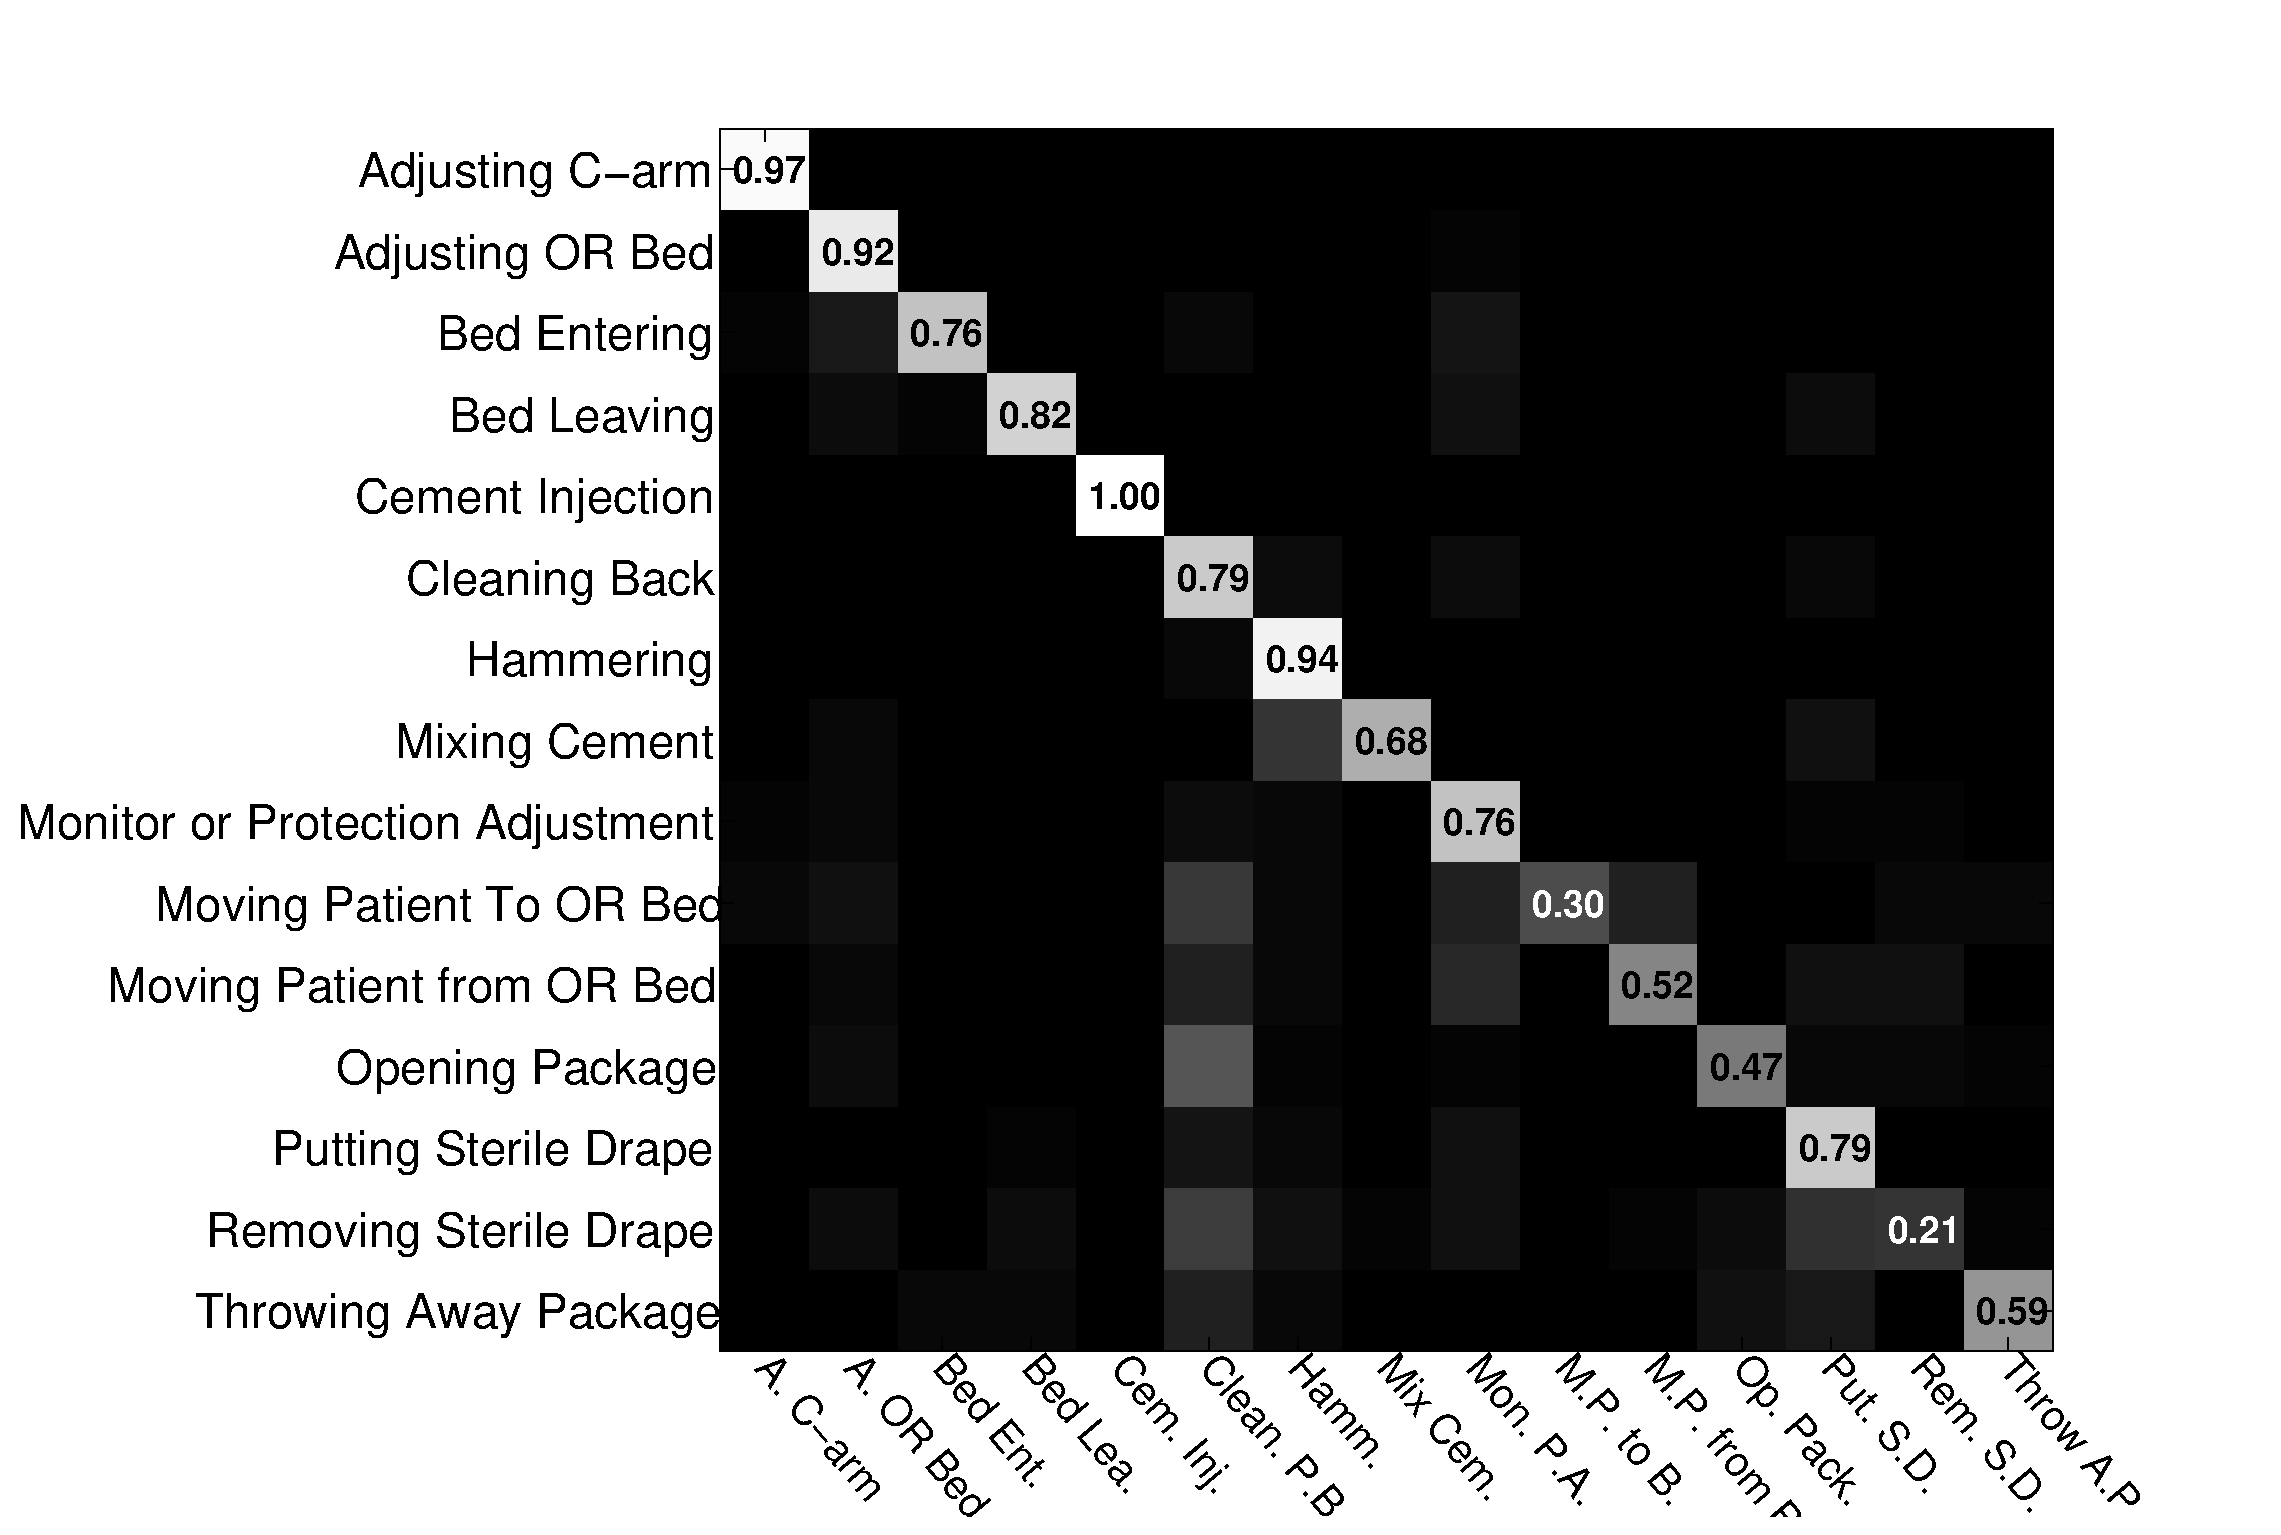
\includegraphics[width=0.7\linewidth]{figures/combination-onemodel}
%\caption{Confusion matrix of one-model approach using combination of the features}
\end{figure}

\begin{center}
{\small  Confusion matrix of one-model approach using combination of the features}
\end{center}

\end{block}

%----------------------------------------------------------------------------------------
%	CONCLUSION
%----------------------------------------------------------------------------------------

\begin{block}{Conclusion \& Future Works}
% 	In this paper, a voting scheme approach is proposed to address the problem of activity recognition in an operating room using a multi-view RGBD camera system. The 4D spatio-temporal space is divided into smaller local patches using a data-driven non-rigid layout by \cite{c1} which also helps with sparse interest points. A two-level classification strategy is introduced, i.e., learning the probability votes and learning the weights. Furthermore, two different classification approaches are compared using two-level classification: one-model and multi-model. The one-model approach performed better than the multi-model. Voting scheme showed promising results with 83.1\% accuracy.

%     The current STIP detection is based on movements occur in the video clips where the detection is in the borders of the action. Hence, the detected interest points are sparse and ignore the information from stationary parts of the videos. Additionally, the BoW approach is another limit which encodes the features into sparse representation. It would be interesting to incorporate extraction of dense features and different feature encoding approaches. Since the voting scheme uses local parts of 4D spatio-temporal space, it would be interesting to use the voting scheme to recognize concurrent activities.

% • Proposed method provides accurate segmentation
% with accelerated speed.
% • Proposed patch creation allowed inclusion
% of all priori.
% • Hierarchical pruning gives better results.
% • Proposed Search Optimization and Integration
% with Optimized Match makes it computationally
% efficient.
% • Validation against multi-class open dataset.
% • Segmentation of subfields can be attempted.
% • Elastic Net(EN)[3] and Group Lasso [2]
% could be explored.
% • Robust pre-selection technique with GPU
% implementation can increase speed.

\begin{itemize}
% \item Data-driven non-rigid layout creates informative 4D spatio-temporal patches
\item The data-driven non-rigid 4D spatio-temporal patches are informative for activity recognition.

\item Two-level classification is required to learn patch weights and their contribution.

\item Because it sees more data more data, the one-model approach performs better than the multi-model approach.

\item The voting scheme shows promising results with 83.1\% accuracy.

\item The current interest point detection is based on movements, sparse and ignore the information from stationary parts.

\item It would be interesting to incorporate the voting scheme for concurrent activity recognition

\end{itemize}

\end{block}

%----------------------------------------------------------------------------------------
%	REFERENCES
%----------------------------------------------------------------------------------------

\begin{block}{References}
        
\nocite{*} % Insert publications even if they are not cited in the poster
\small{\bibliographystyle{unsrt}
\bibliography{sample}}

\end{block}

%----------------------------------------------------------------------------------------
%	ACKNOWLEDGEMENTS
%----------------------------------------------------------------------------------------

% \begin{block}{Acknowledgments}

% \begin{itemize}
% \item Nam mollis tristique neque eu luctus. Suspendisse rutrum congue nisi sed convallis. Aenean id neque dolor. Pellentesque habitant morbi tristique senectus et netus et malesuada fames ac turpis egestas.
% \end{itemize}

% \end{block}

%----------------------------------------------------------------------------------------
%	CONTACT INFORMATION
%----------------------------------------------------------------------------------------

% \setbeamercolor{block title}{fg=black,bg=orange!70} % Change the block title color

% \begin{block}{Contact Information}

% \begin{itemize}
% \item Web: \href{http://www.university.edu/smithlab}{http://www.university.edu/smithlab}
% \item Email: \href{mailto:john@smith.com}{john@smith.com}
% \item Phone: +1 (000) 111 1111
% \end{itemize}

% \end{block}

%----------------------------------------------------------------------------------------

\end{column} % End of the second column

\begin{column}{.015\textwidth}\end{column} % Empty spacer column

\end{columns} % End of all the columns in the poster

\begin{center}
\includegraphics[scale=0.07]{figures/camma_logo_tr}\vspace{50 mm}
%\hspace*{\fill} 
\includegraphics[scale=4]{figures/icube}\vspace{50 mm}
%\hspace*{\fill} 
\includegraphics[scale=1]{figures/unistraTransparent}
\end{center}

\end{frame} % End of the enclosing frame

\end{document}